\part{Introdution : généralités et contexte} % (fold)
\label{prt:introduction_ _théorique_}
	
	\section{BCI} % (fold)
	\label{sec:intro_bci}
	
	BCI: Brain Computer Interface (ou Interface Cerveau-Machine en français).
	Aussi appelée Interface Neuronale Directe (abrégée IND), il s'agit d'une interface de communication directe entre un cerveau et un composant externe (généralement un ordinateur).

	
	\section{EEG} % (fold)
	\label{sec:eeg}
	\begin{figure}[h!]
			\centering
		    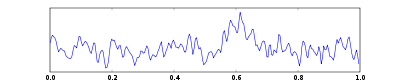
\includegraphics []{figures/eeg_1s_signal.png} \\
		    \captionof{figure}{ci-dessus une seconde de signal EEG}
			\label{fig_eeg_1s}
	\end{figure}
	EEG ou électroencéphalographie est technique de mesure de l'activité électrique du cerveau mesurée à l'aide d'électrodes placées sur le cuir chevelu. L'EEG est un examen indolore est non-invasif comparativement à l'iEEG(électroencéphalographie intracrânienne) qui elle place les électrodes sous la surface du crâne. le signal EEG obtenue est la résultante de la sommation d'un potentiel d'action post-synaptique synchrone issus d'un grand nombre de neurones.
	\begin{figure}
		\centering 
	 	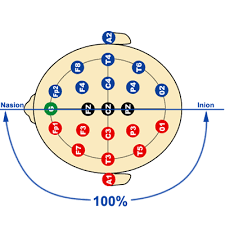
\includegraphics [width=7cm,height=7cm]{figures/captoreeg.png} \\
		\captionof{figure}{positon des capteurs}
		\label{fig_captors}	
	\end{figure}

	% section eeg (end)
	
	% section bci (end)

	\section{Généralités} % (fold)
	\label{sec:généralité}
	
	Ici, certains concepts clés doivent être définis pour comprendre en quoi consiste notre projet: 
	\subsection{Les réseaux de neurones} % (fold)
	\label{sub:les_réseaux_de_neurones}
	 Les réseaux de neurones sont un un modèle de calcul représentant schématiquement les réseaux de neurones biologiques. C'est à celui-ci que 
	l'on va imposer l'apprentissage d'un échantillon de données. Pour cela, nous allons 
	utiliser l'algorithme du gradient, le gradient étant, en mathématiques, un vecteur qui
	 représente la variation d'une fonction en fonction de la variation de ses paramètres. Tout
	  comme nous, le réseau de neurones n'est pas parfait et fera des erreurs lors de son 
	  apprentissage. Il faudra donc utiliser la rétro-propagation du gradient qui est un algorithme 
	  servant à corriger les erreurs du réseau de neurones pour qu'il ne lest reproduise pas.
	% subsection les_réseaux_de_neurones (end)

	\subsection{Notions en liaison avec BCI} % (fold)
	\label{sub:notion_lien}
	Certaines notions sont importantes à connaître lorsque l'on s’intéresse au BCI, entre autre le SSVEP  et le P300. ce sont tout les deux des réponses naturels à une stimulation visuelle. Pour le SSVEP, la réponse est détectée lors d'une stimulation visuelle lorsque la rétine est excitée par une stimulus visuel dont la fréquence d'affichage est entre 3.5Hz et 75Hz. Le P300 par contre 
	est une réponse qui apparaît 300ms après stimulation visuelle. 
	% subsection interface_type_ssvep (end)
	
	% section généralité (end)

	\section{Contexte} % (fold)
	\label{sec:contexte}
	
	   Dans le cadre de ce projet, nous devions développer un réseau de neurones afin de contrôler 
	   automatiquement les activités cérébrales d'un sujet. Ainsi, le système pourrait nous dire grâce au signal EEG
	    du patient quelle activité il est entrain de faire ou bien quelle son état. 
	   Notre système pourrait donc par exemple connaître l'activité d'un malade d'Alzheimer tel que : 
	   \begin{itemize}
	   	\item[-] la lecture;
		\item[-] l'attention sur un film;
		\item[-] l'écriture;
		\item[-] la discussion;
		\item[-] le repos.
	   \end{itemize}
	
	
	
	
		% Contexte et Problématique 
	% section contexte (end)

% part introduction_ _théorique_ (end)